\section{Результаты}
\newcommand{\mannwhitni}{{\footnotesize Значимость отличия выборок по критерию Манна-Уитни: ns $P>0.05$, * $P\leq 0.05$, ** $P\leq 0.01$, *** $P\leq 0.001$}}

\paragraph{Базовые частотные модели} Наши предикторные данные мы обработали разными статистическими методами для получения точностей для сравнения. Были использованы простейшие модели -- частотные, Марковские модели от 1 до 11 порядка. Число параметров марковской модели 11 порядка приближается к числу нуклеотидов в геноме \emph{E.coli}.

Точность предсказания растет в повышением порядка модели, но и число параметров растет экспоненциально. Также модель более высокого порядка специфична к геному организма, на котором она обучена, так как предикторные области большой длины для марковской модели могут не встречаться в геноме, и происходит уже выучивание паттернов последовательности генома.

\begin{table}[h]
\label{table:baselines} \graytable
\caption{Точности предсказания, полученные различными математическими моделями.}
\newcolumntype{M}{>{$}l<{$}}
\begin{tabular}{l >{$}c<{$} >{$}l<{$}}
	Метод &  \text{Точность, \%} & \text{Число параметров} \\
	\thinrule
	Предсказание по частотам во всем геноме & 25.7 & 4\\
	 \verythinrule
	по частоте в предикторной области 12 нуклеотидов & 26.3 & 4\\
	\verythinrule
	по частоте в предикторной области 24 нуклеотидов & 26.5 & 4\\
	\verythinrule
	
\end{tabular}
	
\end{table}



\paragraph{Зависимость от размера предикторной области.} Была исследована зависимость качества предсказания нуклеотида от размера использованной предикторной области. Простейшие архитектуры нейронных сетей (две полносвязных модели, сверточная с разным размером сверточного фильтра) были обучены и протестированы на 30 датасетах. Полученные распределения точности приведены на рисунке \ref{fig:size}. Для всех моделей наблюдается увеличение точности при увеличении размера предикторной области, что подтверждается статистическим критерием Манна-Уитни.

Предикторная область большего размера содержит больше информации, от которой может зависеть следующий нуклеотид. Тем не менее при геометрическом увеличении размера области качество растет практически линейно. Из этого можно сделать вывод о том, что более далекие нуклеотиды слабее влияют на предсказываемую позицию.


\begin{figure*}[h] % two pictures
	\centering
	\begin{subfigure}[t]{0.48\linewidth}
%		\caption{{\bfseries DNN model 1} \\* Полносвязная однослойная модель}
		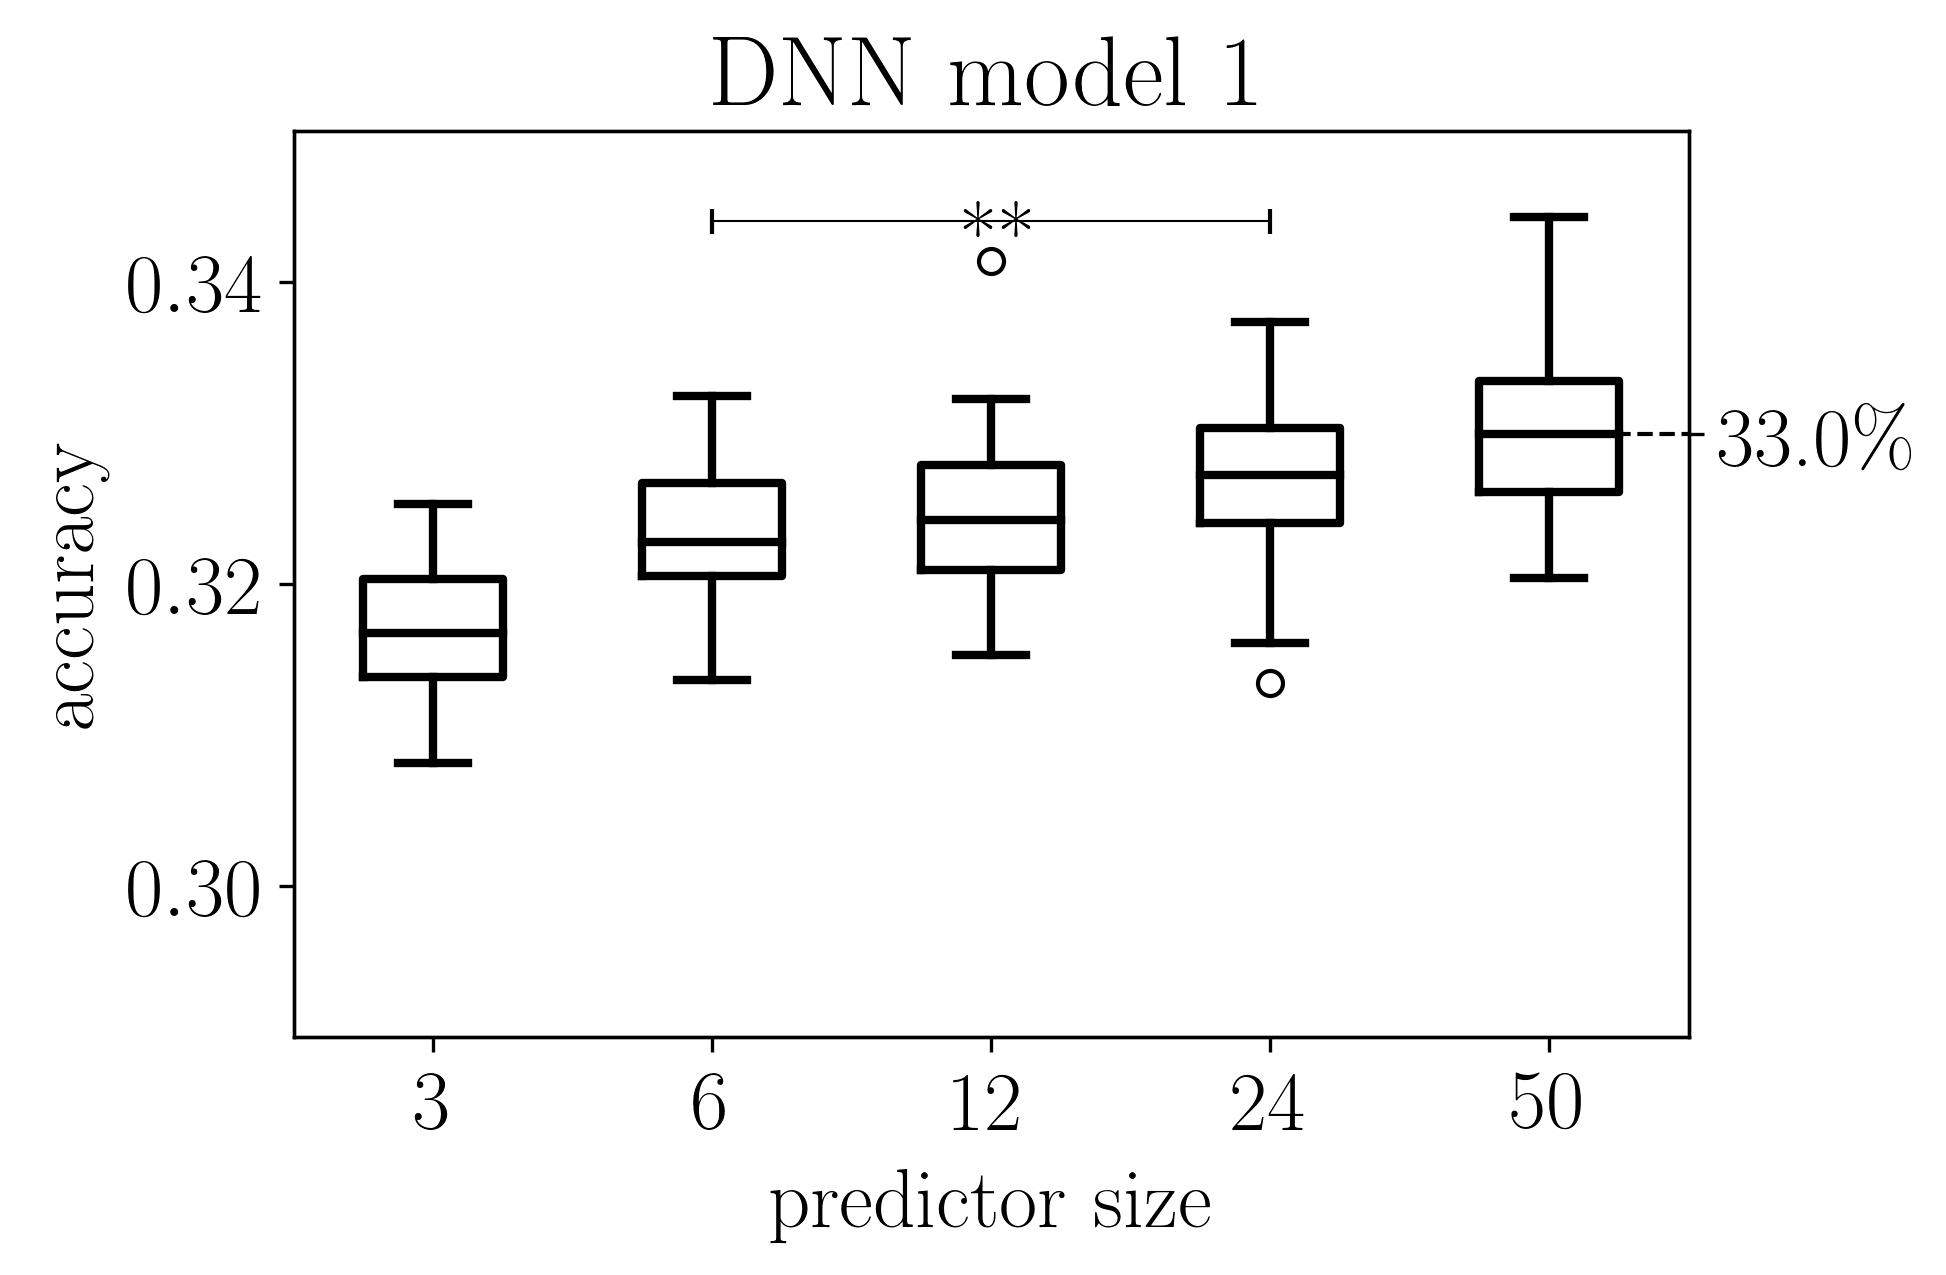
\includegraphics[width = \textwidth]{pics/dnn_model_1_all_runs_p1_ecoli_100000_10000_all_0.png}
		\label{fig:alpha}
	\end{subfigure}
	\begin{subfigure}[t]{0.48\linewidth}
%		\caption{mm}
		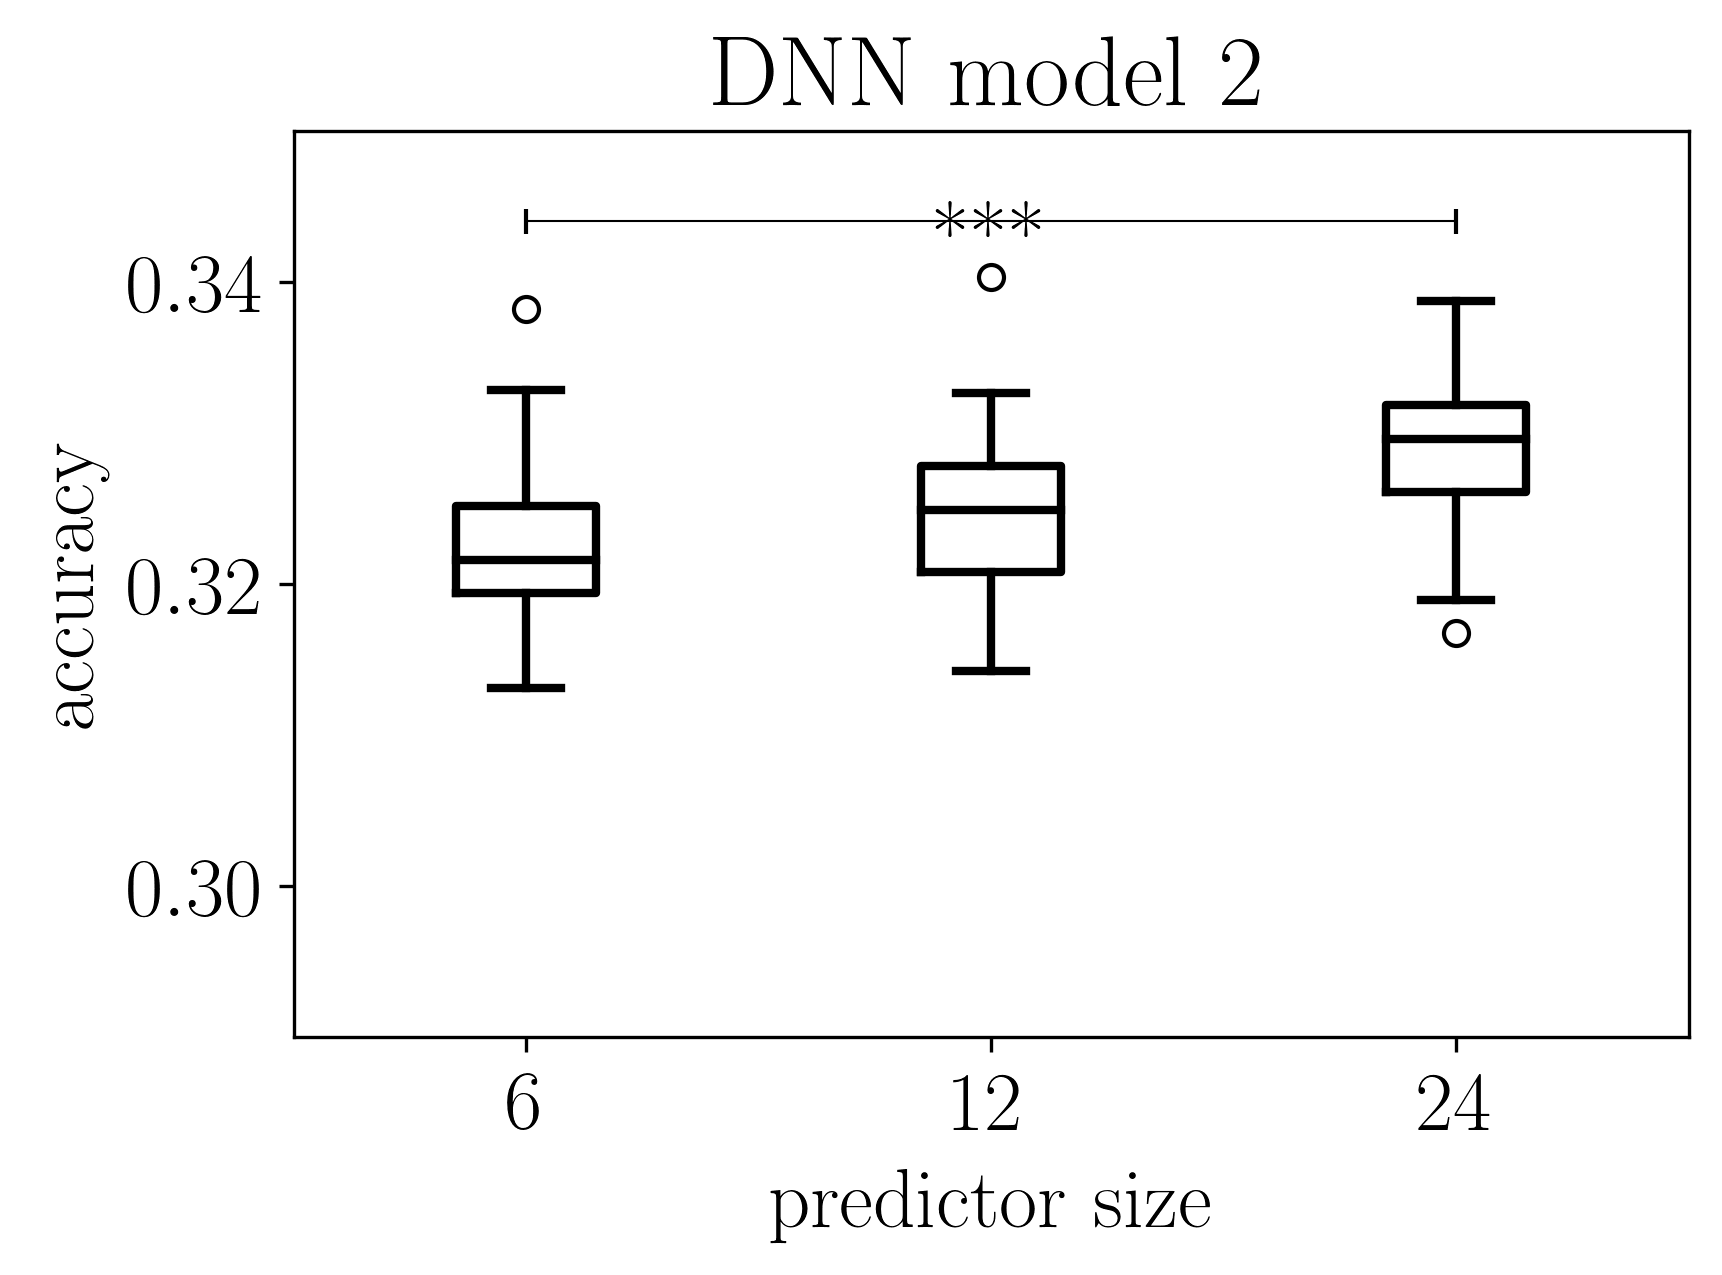
\includegraphics[width = \textwidth]{pics/dnn_model_2_all_runs_p1_ecoli_100000_10000_all_0.png}
			\label{fig:alpha}
	\end{subfigure}
	\begin{subfigure}[]{0.48\linewidth}
%		\caption{{\bfseries CNN model 1} \\* Сверточная однослойная модель }
		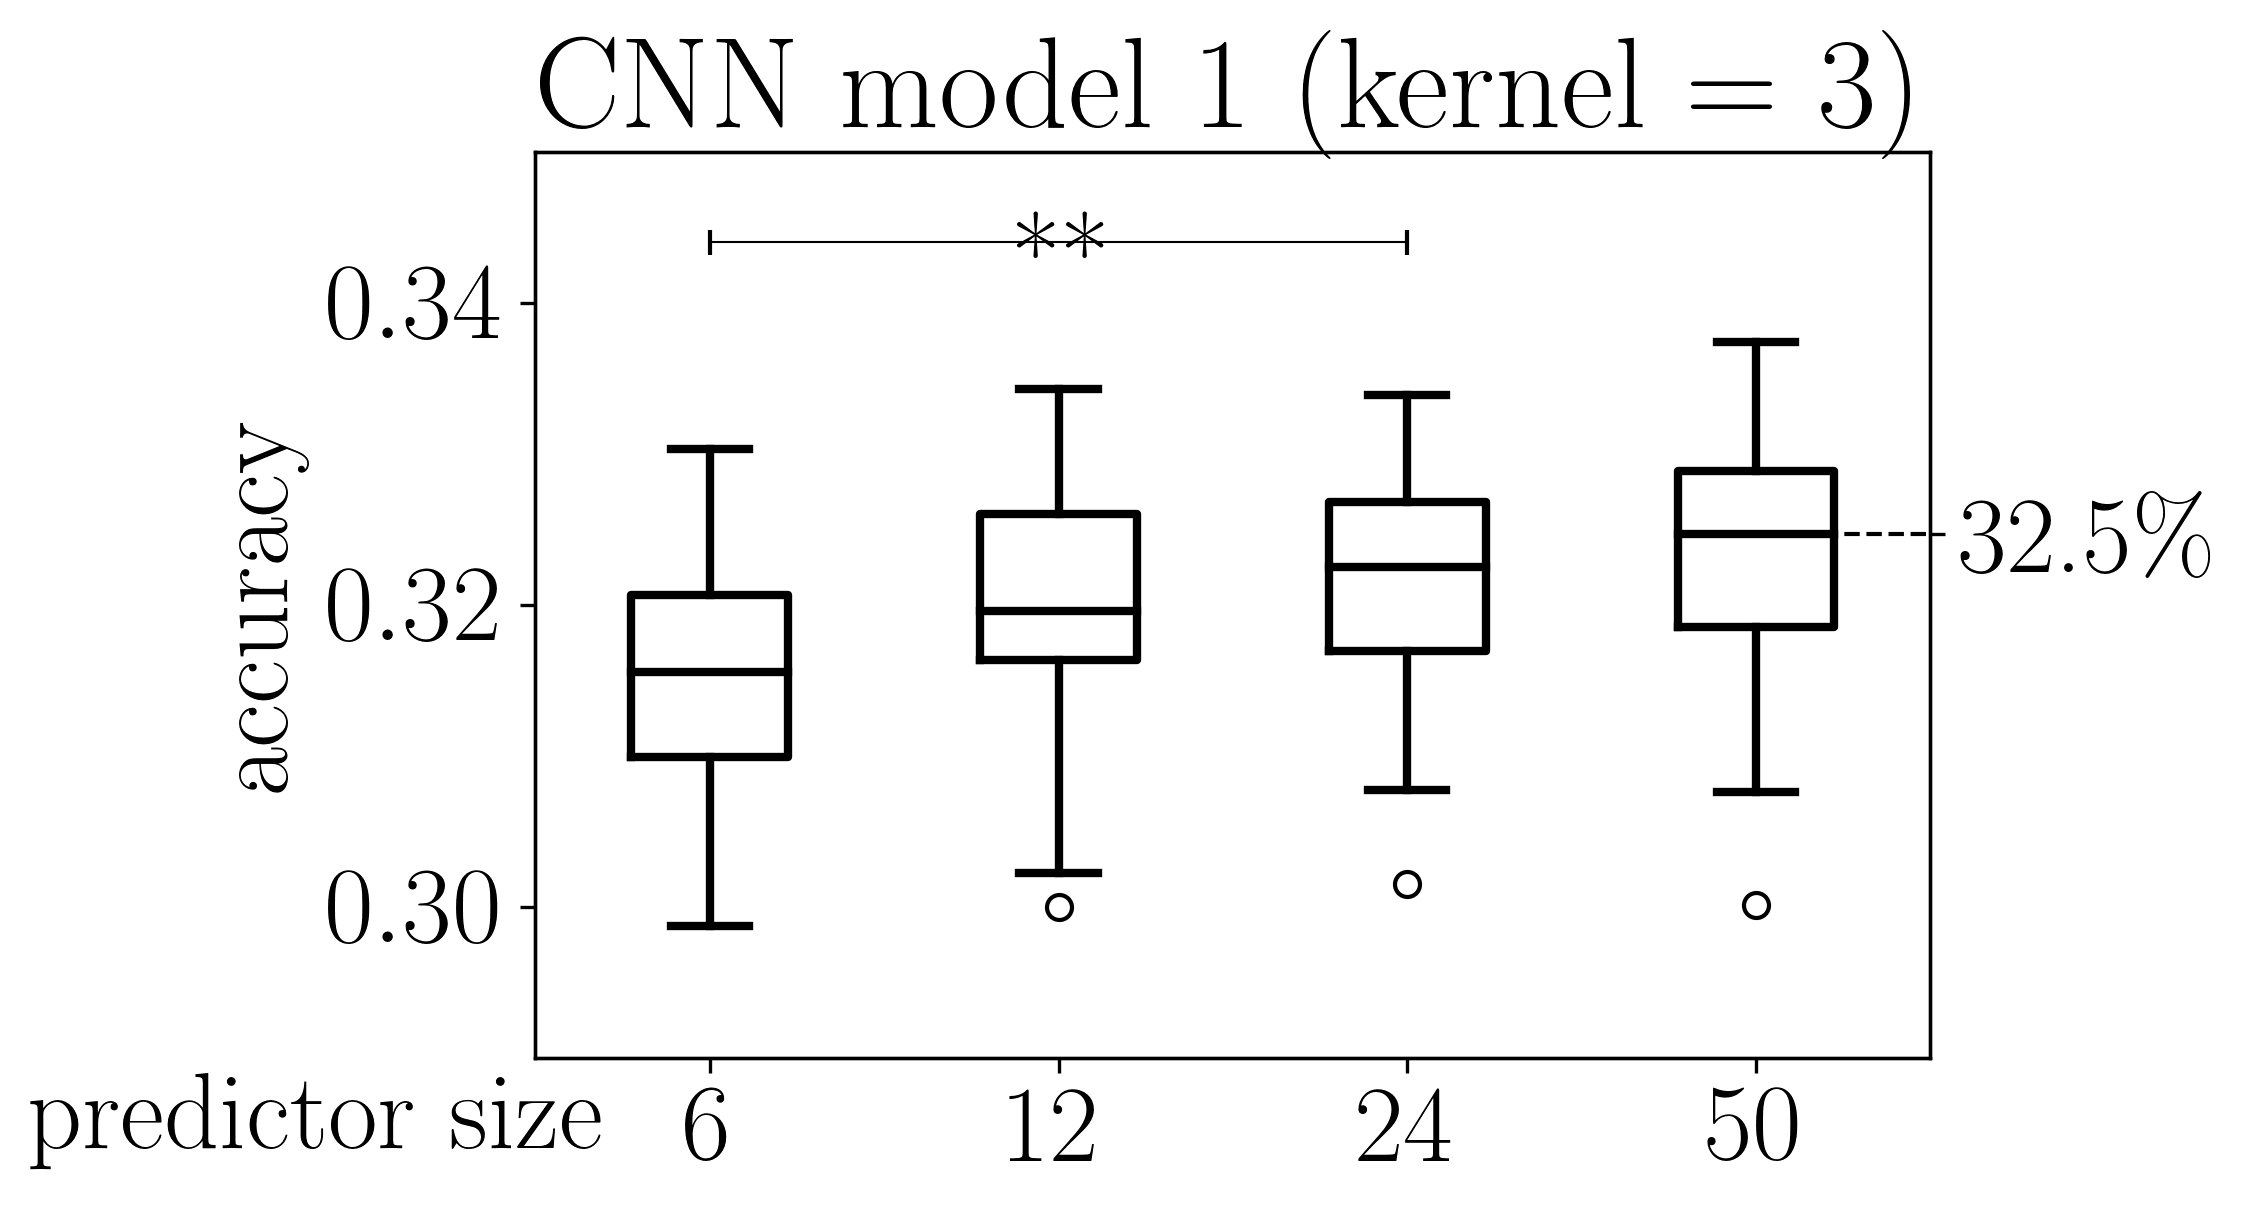
\includegraphics[width = \textwidth]{pics/cnn_model_1_all_runs_p1_ecoli_100000_10000_all_0.png}
		\label{fig:beta}
	\end{subfigure}
	\begin{subfigure}[]{0.48\linewidth}
%		\caption{{\bfseries CNN model 1} \\* Сверточная однослойная модель }
		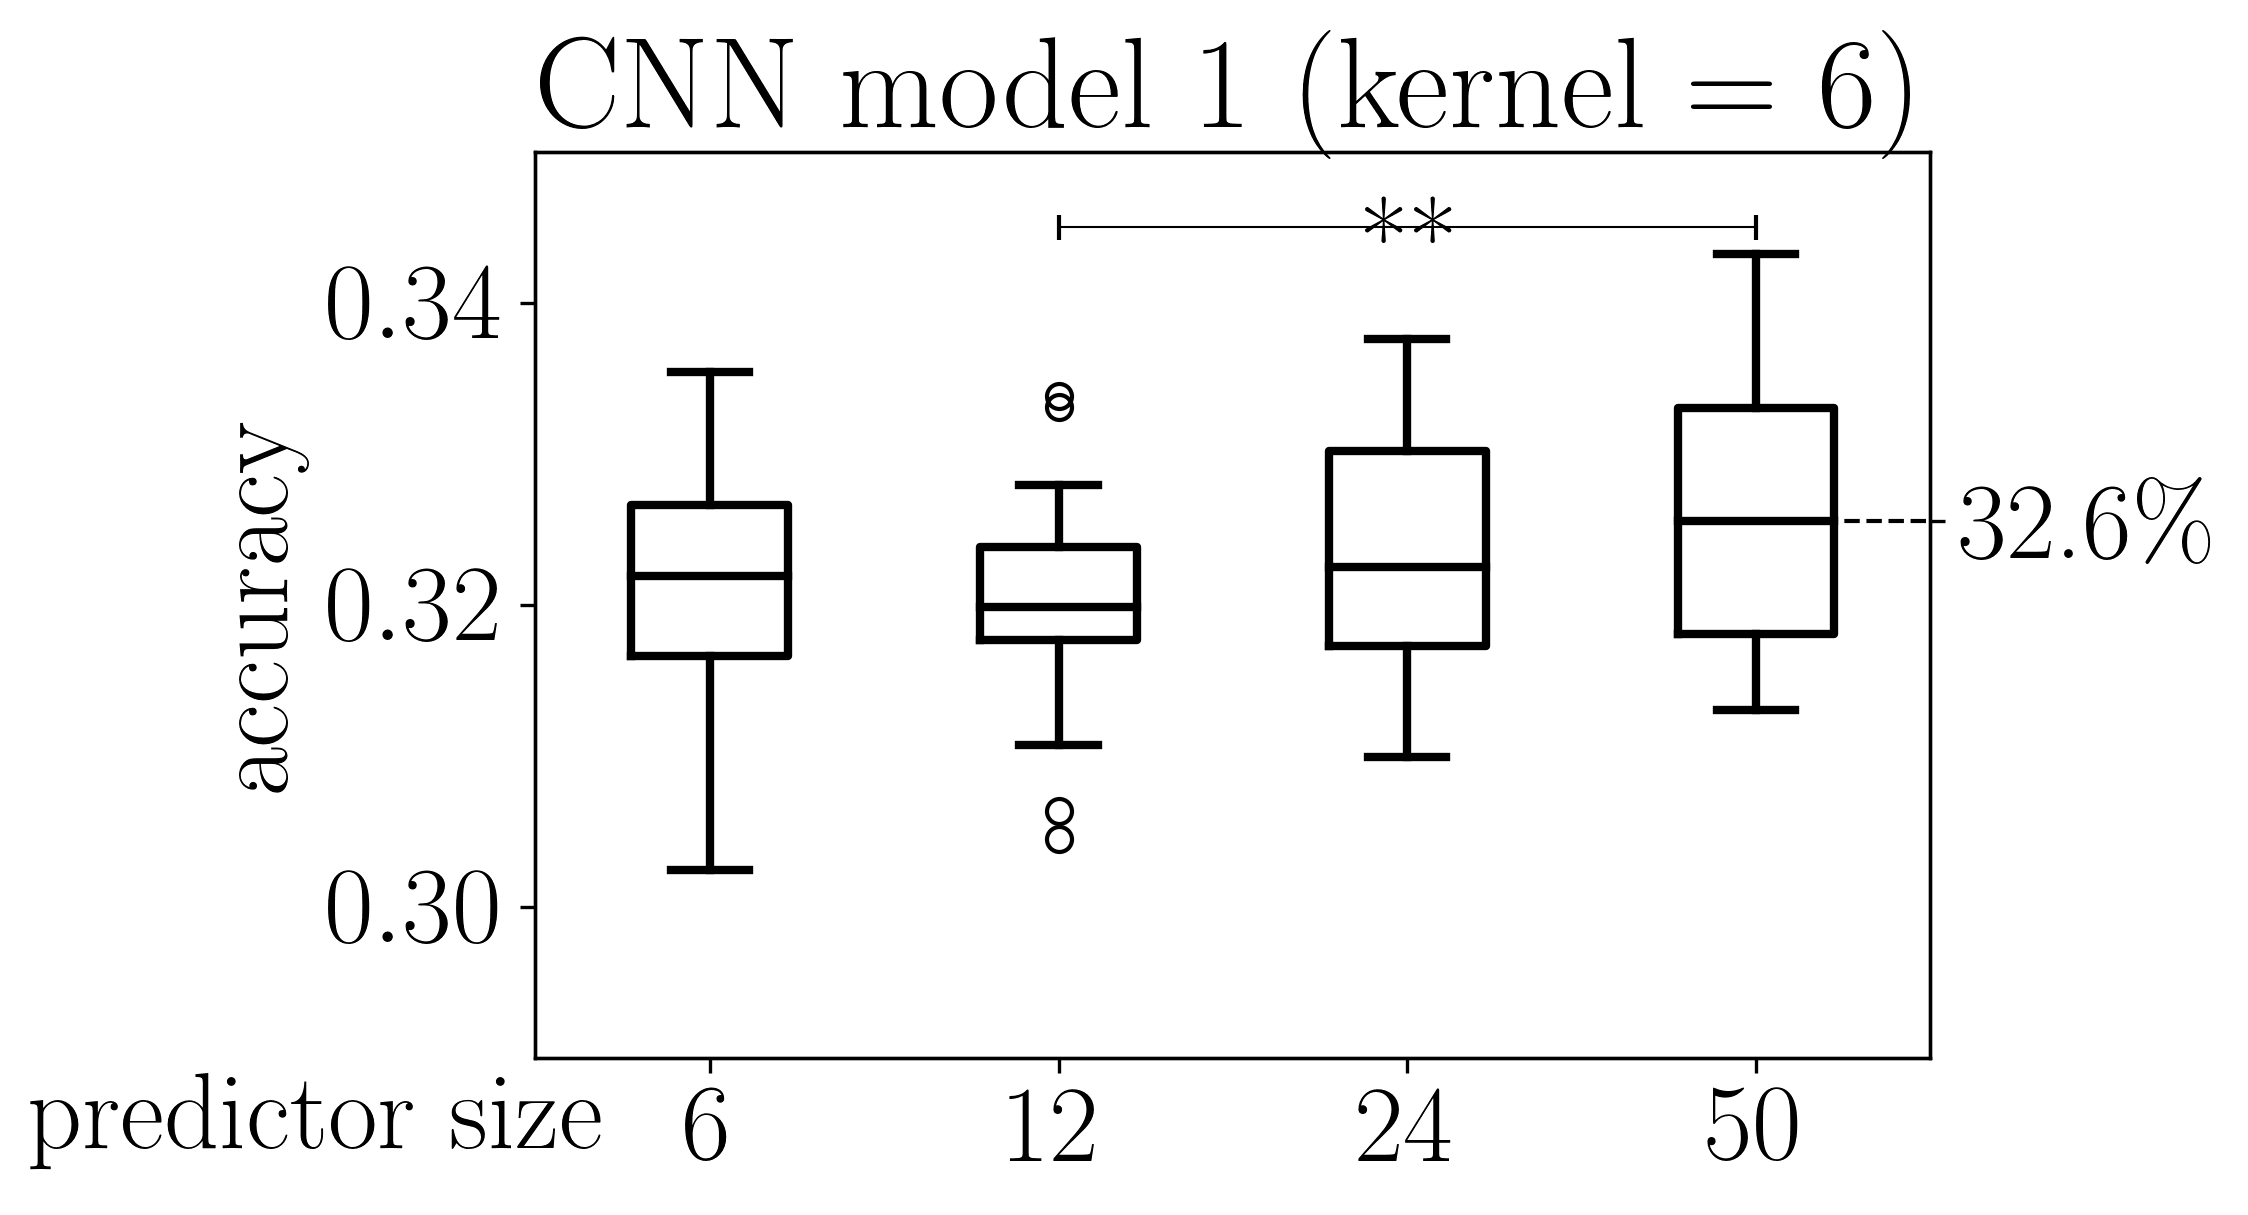
\includegraphics[width = \textwidth]{pics/cnn_model_2_all_runs_p1_ecoli_100000_10000_all_0.png}
		\label{fig:cnn_2_predictor}
	\end{subfigure}
	\caption{{\bfseries Зависимость точности предсказания от размера предикторной области для различных архитектур.} \\*
	По горизонтальной оси обозначен размер области. По вертикальной оси показано распределение точностей обученной модели в сете из 30 запусков с различными наборами данных.}
	
	\label{fig:size}
	
\end{figure*}

\paragraph{Зависимость от отступа.} Была исследована зависимость качества предсказания от расстояния между предикторной областью и предсказываемым нуклеотидом для двух моделей -- полносвязной и сверточной. 

С увеличением отступа качество предсказания падает, причем резко. Это подтверждает то, что в простых моделях (полносвязных и сверточных с небольшим числом параметров) предсказание основывается на ближайших в предсказываемому нуклеотидах.

\begin{figure*}[h] % two pictures
	\centering
	\begin{subfigure}[t]{0.47\linewidth}
		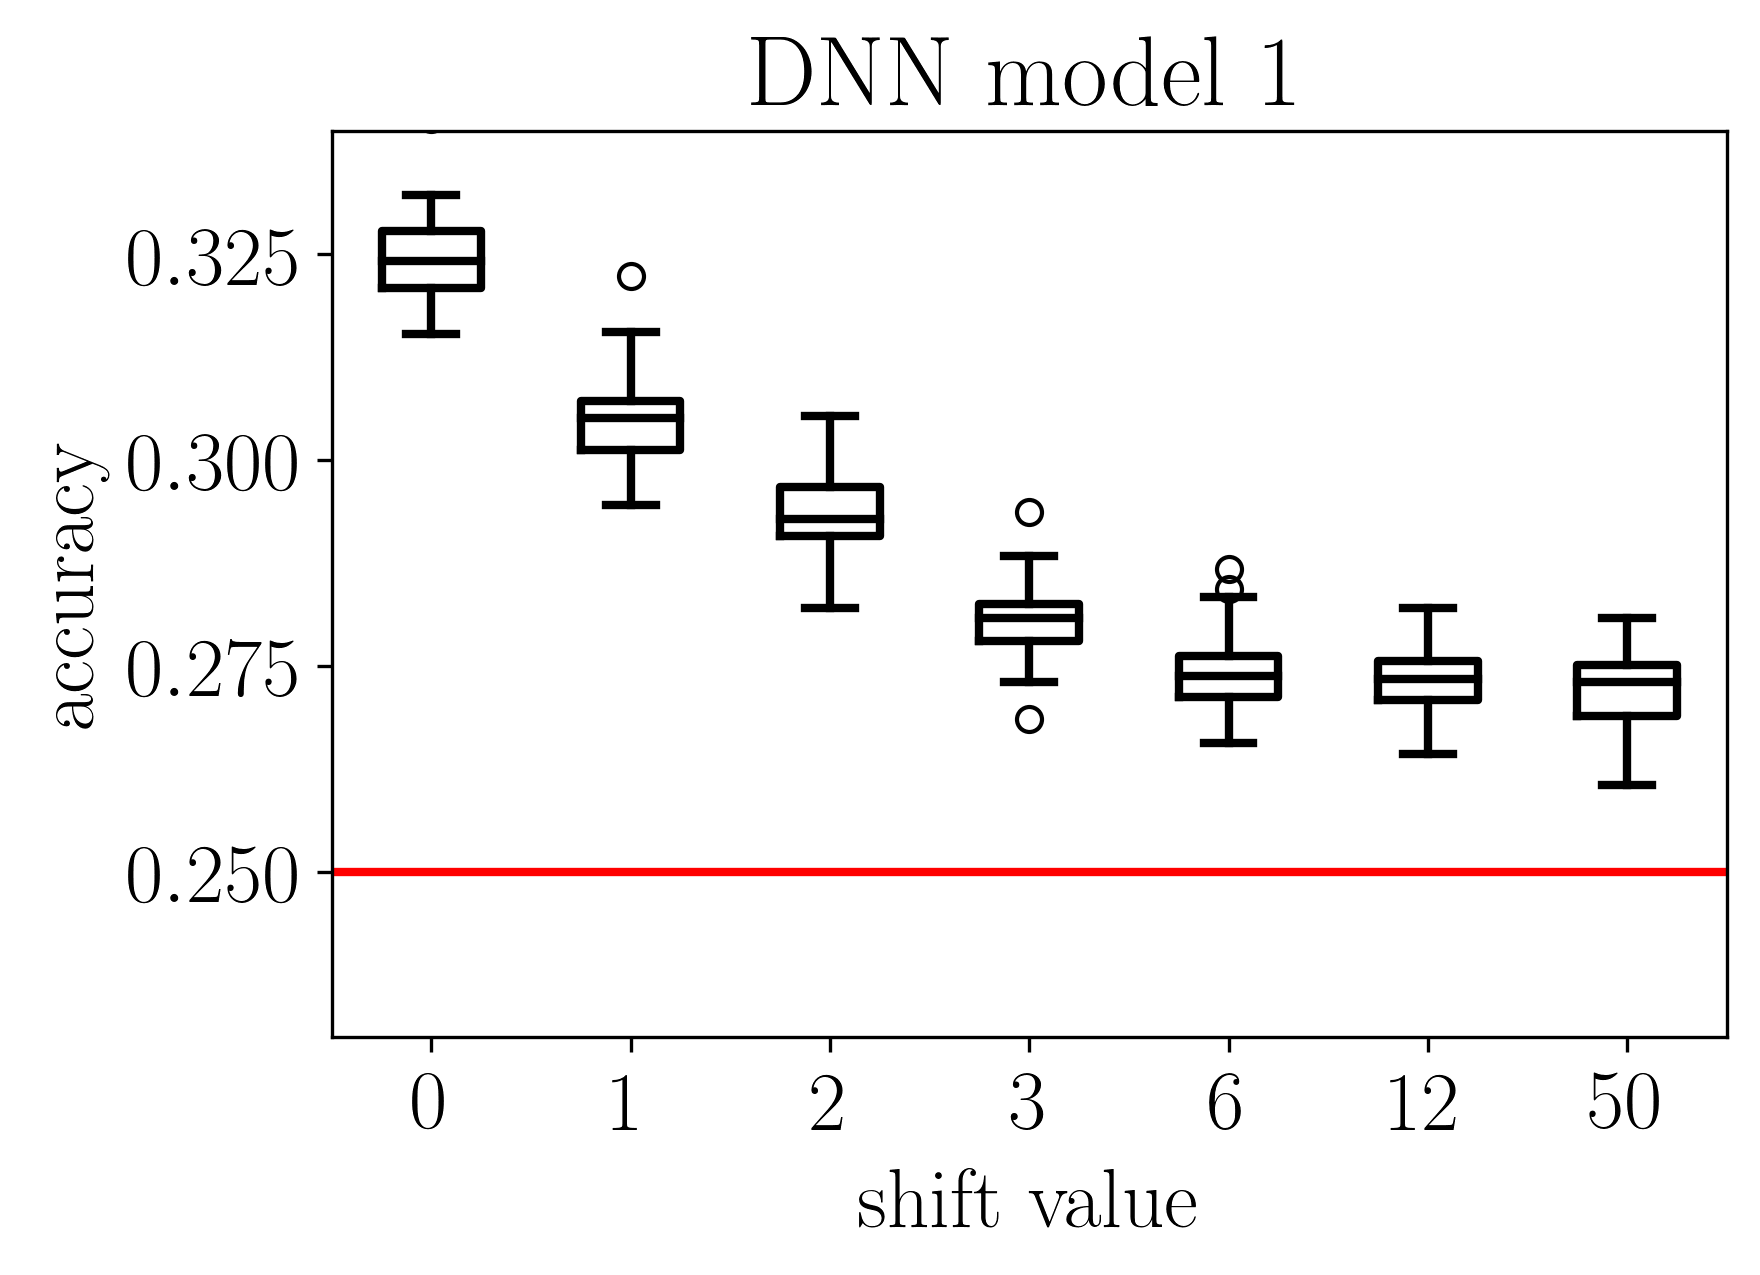
\includegraphics[width = \textwidth]{pics/dnn_model_1_all_runs_p1_ecoli_100000_10000_12_all.png}
		\caption{{\bfseries DNN model 1} \\*
		Полносвязная однослойная модель. Размер предикторной области 12.
		}
		\label{fig:dnn_shift}
	\end{subfigure}
	\begin{subfigure}[t]{0.47\linewidth}
		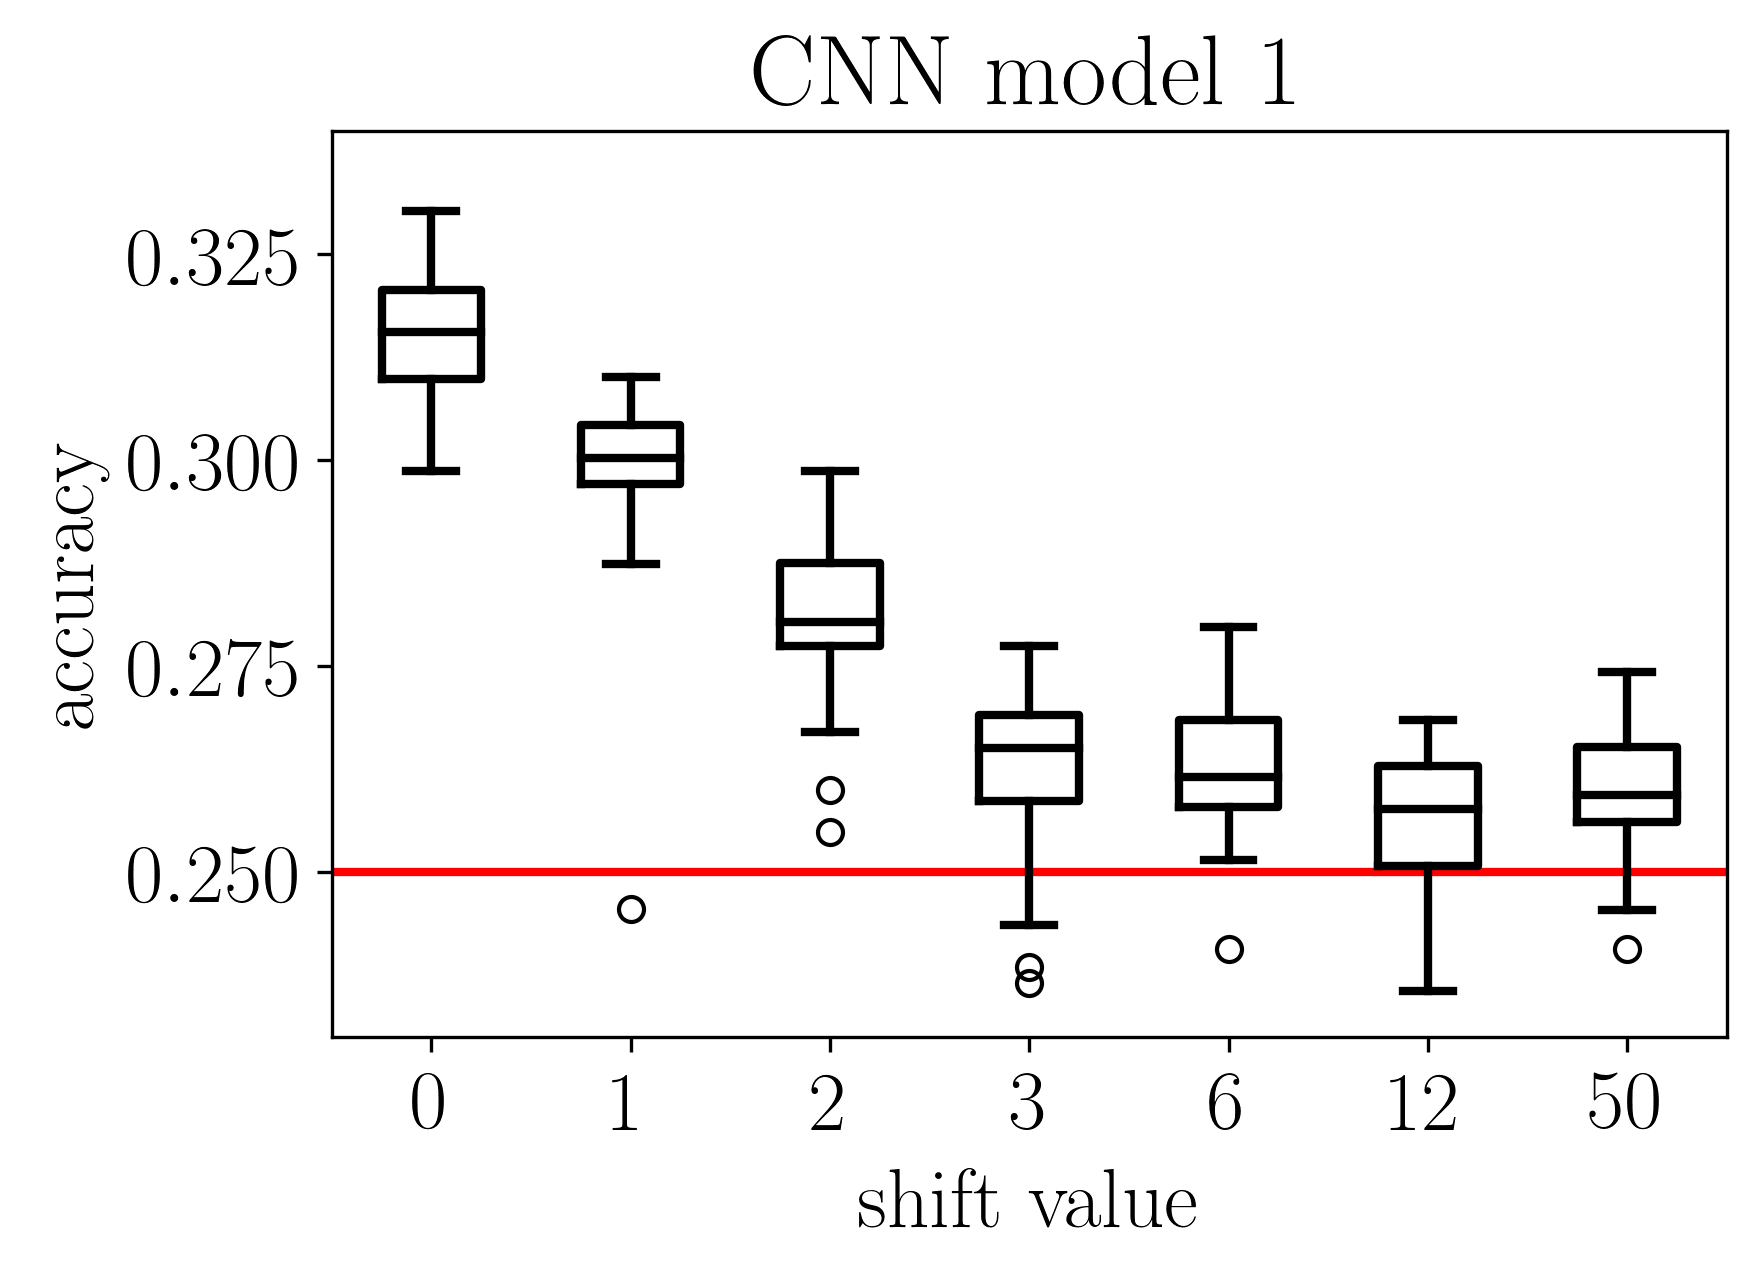
\includegraphics[width = \textwidth]{pics/cnn_model_1_all_runs_p1_ecoli_100000_10000_6_all.png}
		\caption{{\bfseries CNN model 1 (kernel = 3)} \\*
		Сверточная однослойная модель. Размер предикторной области 6.
		}
		\label{fig:cnn_shift}
	\end{subfigure}
	\caption{{\bfseries Зависимость точности предсказания от расстояния между предикторной областью и предсказываемым нуклеотидом (от отступа)  для различных архитектур.} \\*
	По горизонтальной оси обозначен размер отступа. По вертикальной оси показано распределение точностей обученной модели в 30 запусках с различными наборами данных. Горизонтальная линия отмечает точность случайного предсказания 25\%.}	
	\label{fig:shift}
	
\end{figure*}
 
 \paragraph{Сравнение полносвязных моделей.} Мы сравнили между собой полносвязные модели -- с одним (DNN model 1) и двумя слоями (DNN model 2)  на двух типах данных -- предсказание по предикторной области 12 и 24 (рисунок \ref{fig:dnn_test}). Статистически значимой разницы между моделями не наблюдалось.
 
 Полносвязные модели по построению не могут должным образом использовать информацию о близком расположении и последовательности нуклеотидов. В таких моделях предсказание, большей степени, основывается на нуклеотидном составе предикторной области.
 
\begin{figure}[h] % picture
	\centering
	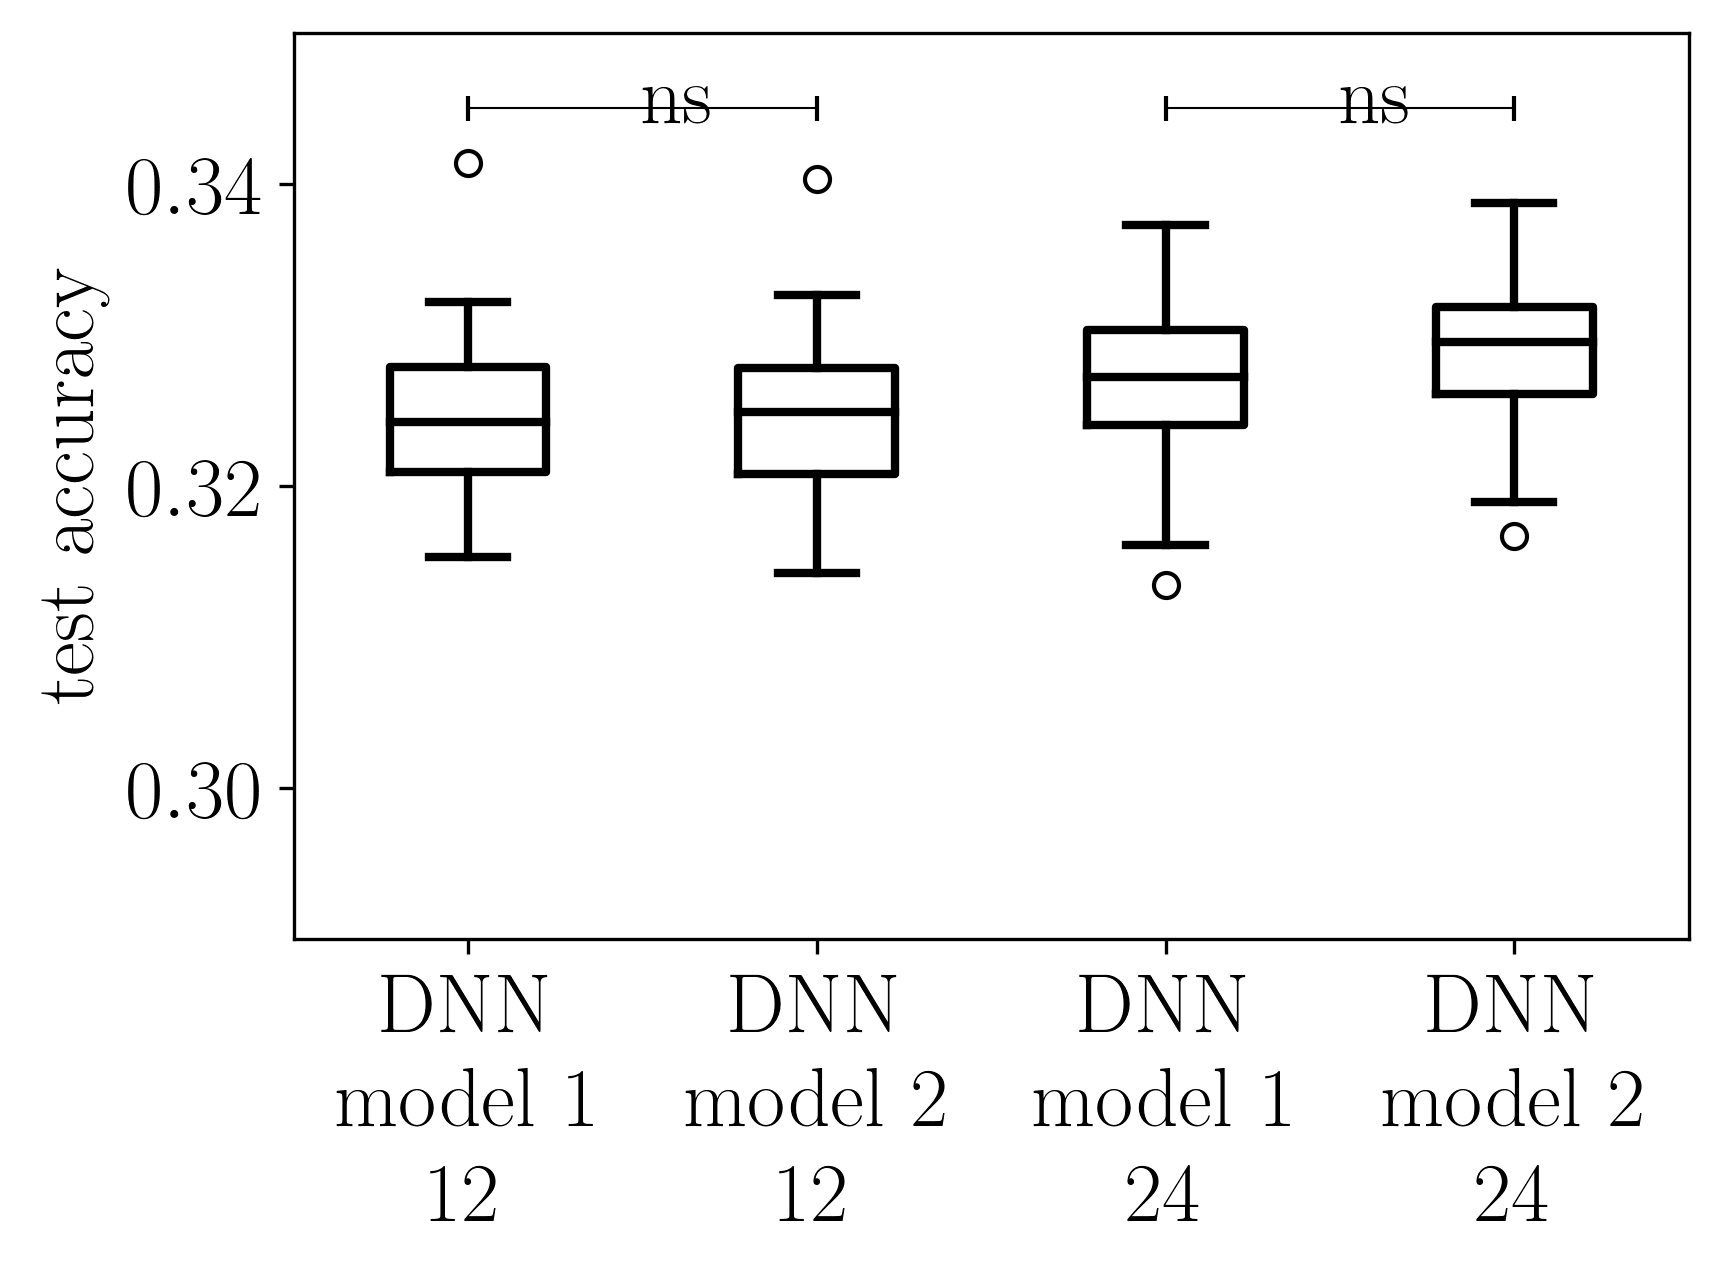
\includegraphics[width = 0.6\textwidth]{pics/dnn_models_all_runs_p1_ecoli_100000_10000_12_0.png}
	\caption{{\bfseries Сравнение полносвязных моделей.} \\* 
		На рисунке показано распределение качестве предсказания полносвязных моделей на двух вариантах данных -- с предикторной областью 12 и 24. В обоих случаях разница в качестве предсказания статистически не значима. \\
		   \mannwhitni }
	\label{fig:dnn_test}	
\end{figure}


\paragraph{Сравнение сверточных моделей.} Мы исследовали несколько вариантов конфигурации сверточного слоя. Результаты тестов приведены на рисунке \ref{fig:cnn_test}.

\input{tables/cnn_comparison}

\paragraph{Рекурретные модели.}
\begin{figure}[h] % picture
	\centering
	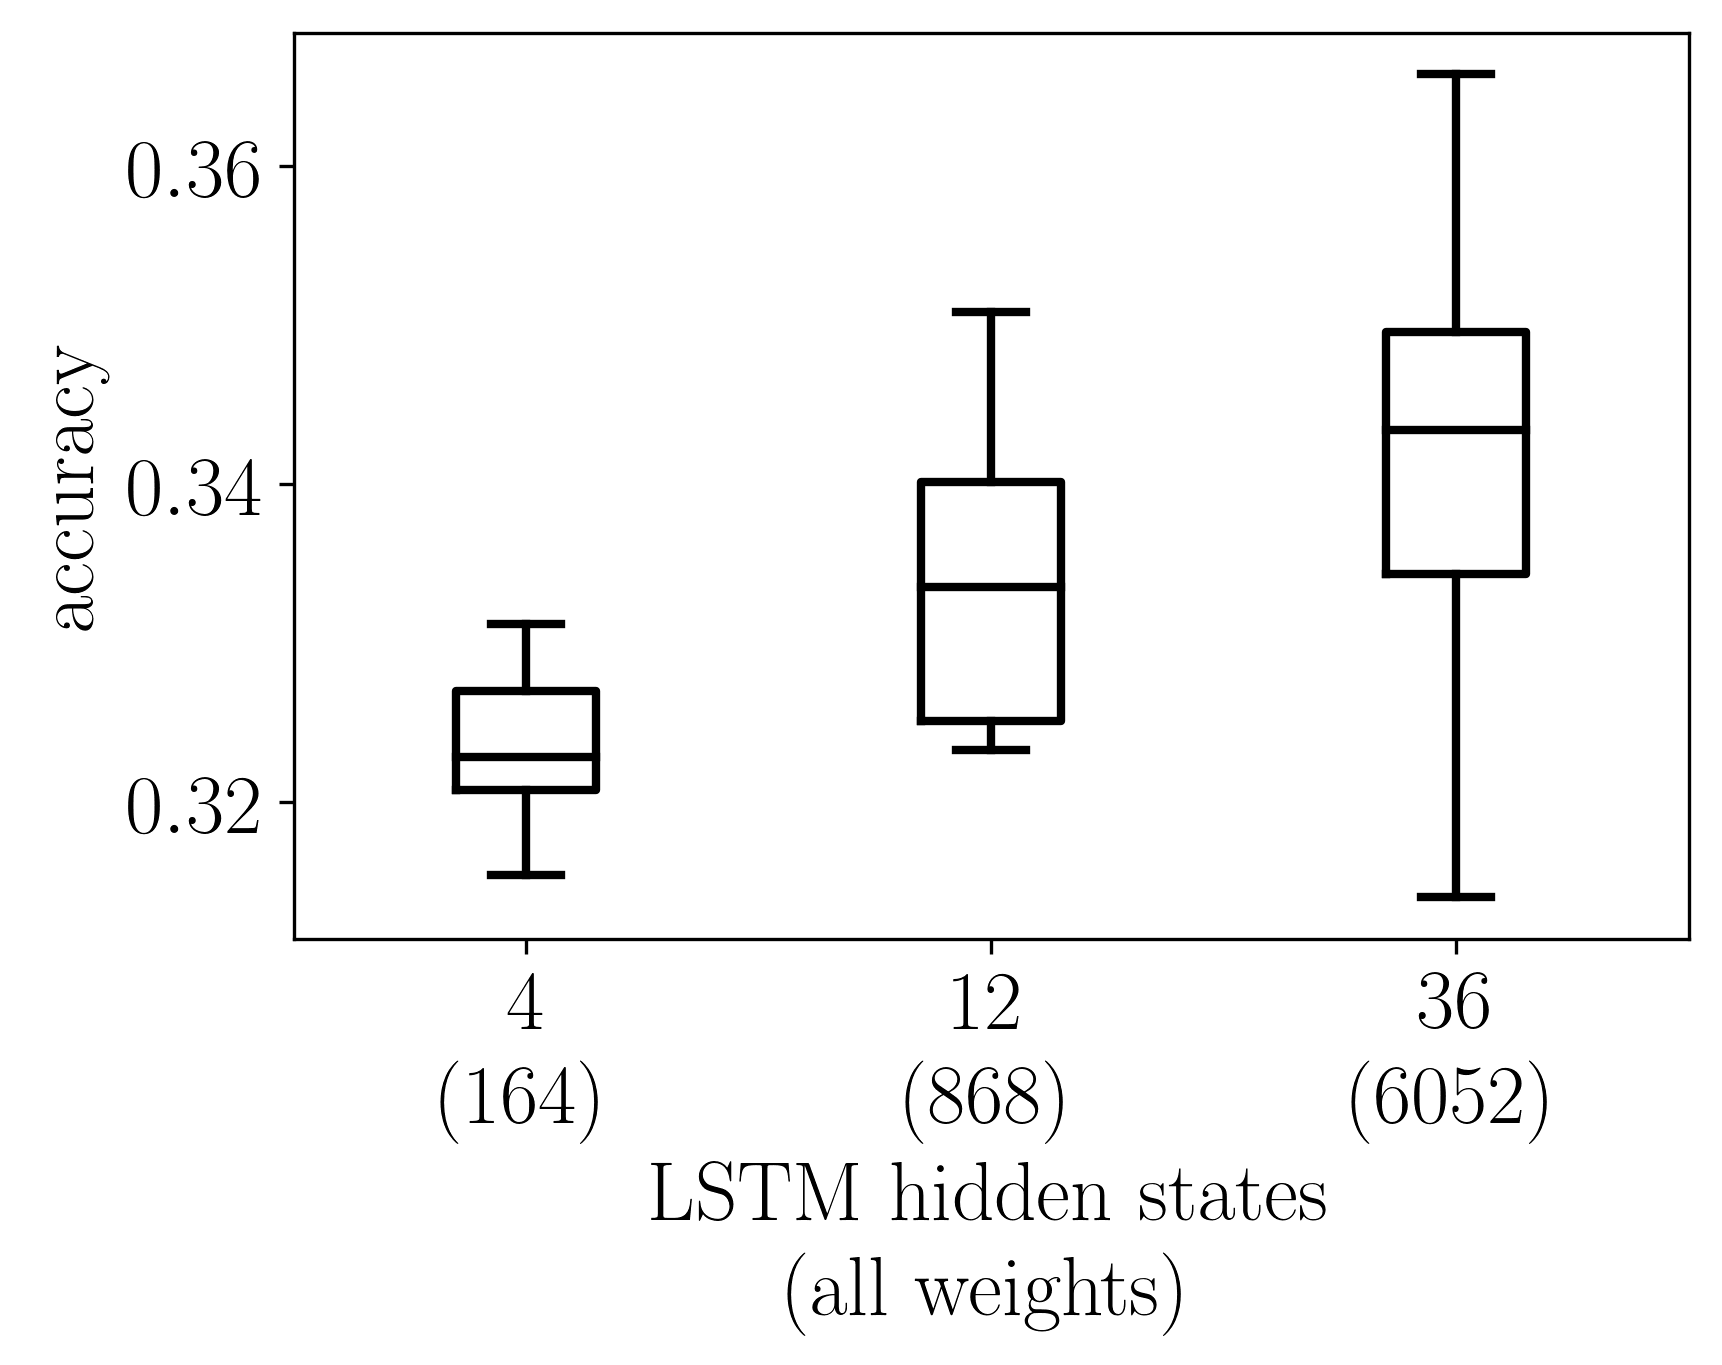
\includegraphics[width = 0.6\textwidth]{pics/rnn_models_all_runs_p1_ecoli_100000_10000_50_0.png}
	\caption{{\bfseries Сравнение рекуррентных моделей.} \\* 
		   \mannwhitni }
	\label{fig:rnn_test}	
\end{figure}

	